\documentclass{beamer}

\usepackage{amsmath, amssymb}
\usepackage{tikz-cd}
\usepackage{xcolor}
\usepackage{graphicx}
\usepackage{capt-of}

\title{MAT434: Theory of Mathematical Statistics}
\author{\textbf{Miraj Samarakkody}}
\institute{Tougaloo College}
\date{04/04/2025}

\begin{document}

\begin{frame}
    \titlepage
\end{frame}



\begin{frame}{Chapter 3}
    \Huge{Continuous Random Variables}
\end{frame}





\begin{frame}{Example A}
    Consider the bivariate density function \[f(x,y)=\dfrac{12}{7}(x^2+xy),~0 \leq x \leq 1,~0\leq y \leq 1.\] Calculate \(P(X>Y)\). 

    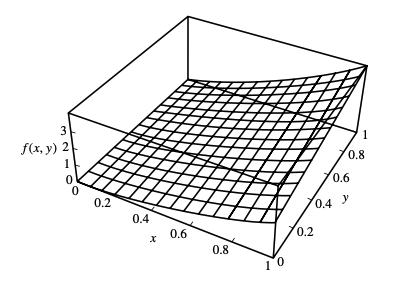
\includegraphics[scale=0.5]{Figures/fig_7.png}


\end{frame}

\begin{frame}{Continuous Random Variables}
    The \textbf{marginal cdf} of \(X\), of \(F_X\), is \begin{align*}
        F_X(x) & = P(X \leq x)\\
        & = \lim_{y \to \infty}F(x,y)\\
        & = \int_{-\infty}^{x} \int_{-\infty}^{\infty} f(u,y)~dy~du
    \end{align*}
    The marginal density of \(X\) is \[f_X(x)=F'_X(x)= \int_{-\infty}^{\infty}f(x,y)~dy\]
\end{frame}


\begin{frame}{Example B}
    Consider the bivariate density function \[f(x,y)=\dfrac{12}{7}(x^2+xy),~0 \leq x \leq 1,~0\leq y \leq 1.\] Find the marginal density of \(X\). 


\end{frame}


\begin{frame}
    \frametitle{Example D}

    Consider the following joint density:
    \[f(x,y)= \begin{cases}
        \lambda^2 e^{-\lambda y}, & 0 \leq x \leq y, ~\lambda >0\\
        0, & \text{elsewhere}
    \end{cases}\] Find the marginal densities. 
    \begin{figure}
        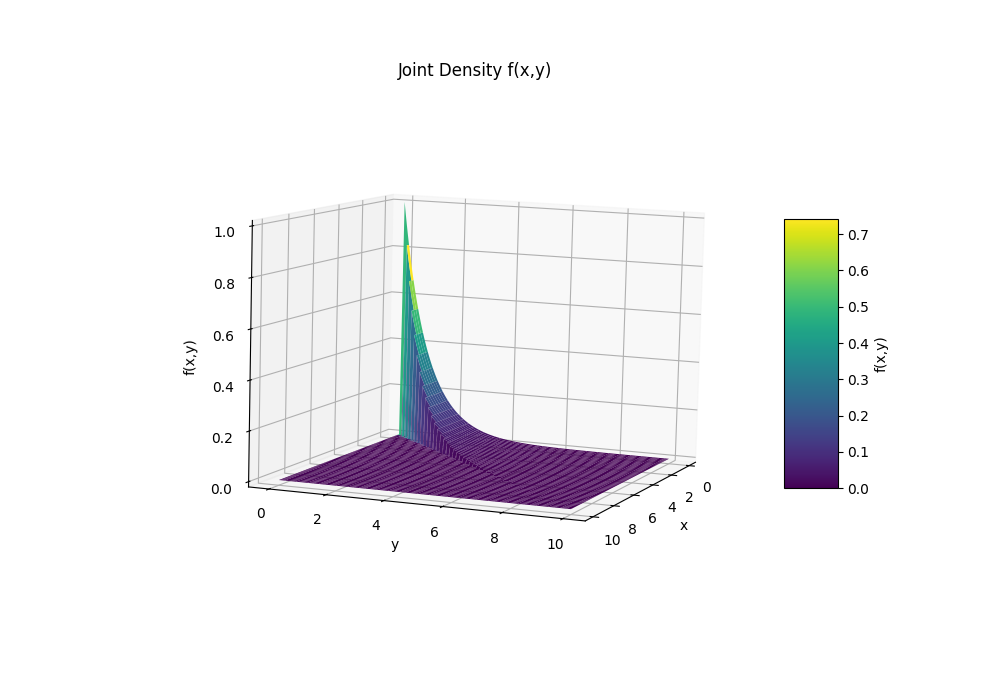
\includegraphics[scale=0.4]{Figures/fig_9.png}
        \captionof{figure}{With \(\lambda=1\)}
    \end{figure}
    

\end{frame}

\begin{frame}{Continuous Random Variables}
    \begin{itemize}
        \item In some applications, it is useful to analyze distributions that are uniform over some region space. 
        \item For example, in the plane, the random point \((X,Y)\) is uniform over a region \(R\), if for any \(A \subset R\), \[P((X,Y) \in A)=\dfrac{|A|}{|R|}\]
    \end{itemize}    
\end{frame}

\begin{frame}{Example E}
    A point is chosen randomly in a disk of radius 1. Since the area of the disk is \(\pi\), \[f(x,y)= \begin{cases}
        \dfrac{1}{\pi} & \text{if }x^2+y^2\leq 1\\
        0, & \text{otherwise}
    \end{cases}\] Find \(F_R(r)\), \(f_R(r)\)  \(f_X(x)\) and \(f_Y(y)\). 
\end{frame}


\begin{frame}{}
    \Huge{Independent Random Variables}
\end{frame}

\begin{frame}{Independent Random Variables}
    \begin{block}{Definition}
        Random variables \(X_1,X_2, X_3, \dots, X_n\) are said to be \textit{independent} if their joint cdf factors into the product of their marginal cdf's:
        \[F(x_1, x_2, \dots, x_n)= F_{X_1}(x_1)F_{X_2}(x_2)\dots F_{X_n}(x_n)\] for all \(x_1, x_2, \dots, x_n\). 
    \end{block}

    This definition holds for both continuous and discrete random variables:
\end{frame}





\end{document}